% This structure conforms to the mcgill university wide thesis guidelines:
% 
% https://www.mcgill.ca/gps/thesis/thesis-guidelines/preparation
% Some parts of it were taken from here, but mostly it is a "from scratch" template with minimal bload and fuzz: https://github.com/juliengs/mcgill-thesis-template
% Author: Maximilian Schiedermeier

\documentclass[12pt,oneside]{book}
\usepackage{graphicx}

% enable onehalfspaceing etc
\usepackage{setspace}

% Make chapter enumeration big and fat
\usepackage{fix-cm}
\usepackage{xcolor}
\usepackage[bf,rm,medium,compact]{titlesec}
\definecolor{gray75}{gray}{0.75}
\newcommand{\hsp}{\hspace{20pt}}
\titleformat{\chapter}[display]{\filleft\Huge\bfseries}{\fontsize{100}{100}\selectfont\textcolor{gray75}\thechapter}{1ex}{}[]%


% Enable non-ugly hyperlinks
\usepackage{blindtext}
\usepackage[hidelinks]{hyperref}




% Some metadata for your generated PDF
\title{Phd Thesis}
\author{Your-First-Name Your-Family-Name}
\date{\today}

% DOCUMENT BEGINS
\begin{document}


% Special command to link to official guidelines:
\newcommand{\mcgillguidelines}{\href{https://www.mcgill.ca/gps/thesis/thesis-guidelines/preparation}{Official McGill Guidelines: }}


% TITLE PAGE
\begin{onehalfspacing}
\pagestyle{empty}
% This title page conforms to the mcgill university wide thesis guidelines:
% https://www.mcgill.ca/gps/thesis/thesis-guidelines/preparation

% Students can request permission to add the official McGill logo to their thesis cover page by submitting this webform: https://www.mcgill.ca/visual-identity/application-use-university-logo-demande-dutilisation-du-logo-de-luniversite


\begin{titlepage}
\begin{center}

\vspace*{0.5cm}


{\bfseries\LARGE  AiMentalAcoustics}
\vspace{0.15cm}

{\bfseries\LARGE  Contactless AI-assistive system to}
\vspace{0.15cm}

{\bfseries\LARGE  recognize, detect, and forecast for mental wellness}
\vspace{1.8cm}

{\large Prasannjeet Singh}
% \\Doctor of Philosophy

% Institution
\vspace{1cm}
% The McGill Logo
% NOTE: YOU HAVE TO ASK FOR PERMISSION TO INTEGRATE THE LOGO. YOU CAN GET IT HERE: https://www.mcgill.ca/visual-identity/application-use-university-logo-demande-dutilisation-du-logo-de-luniversite
\begin{figure}[ht!]
    \centering
    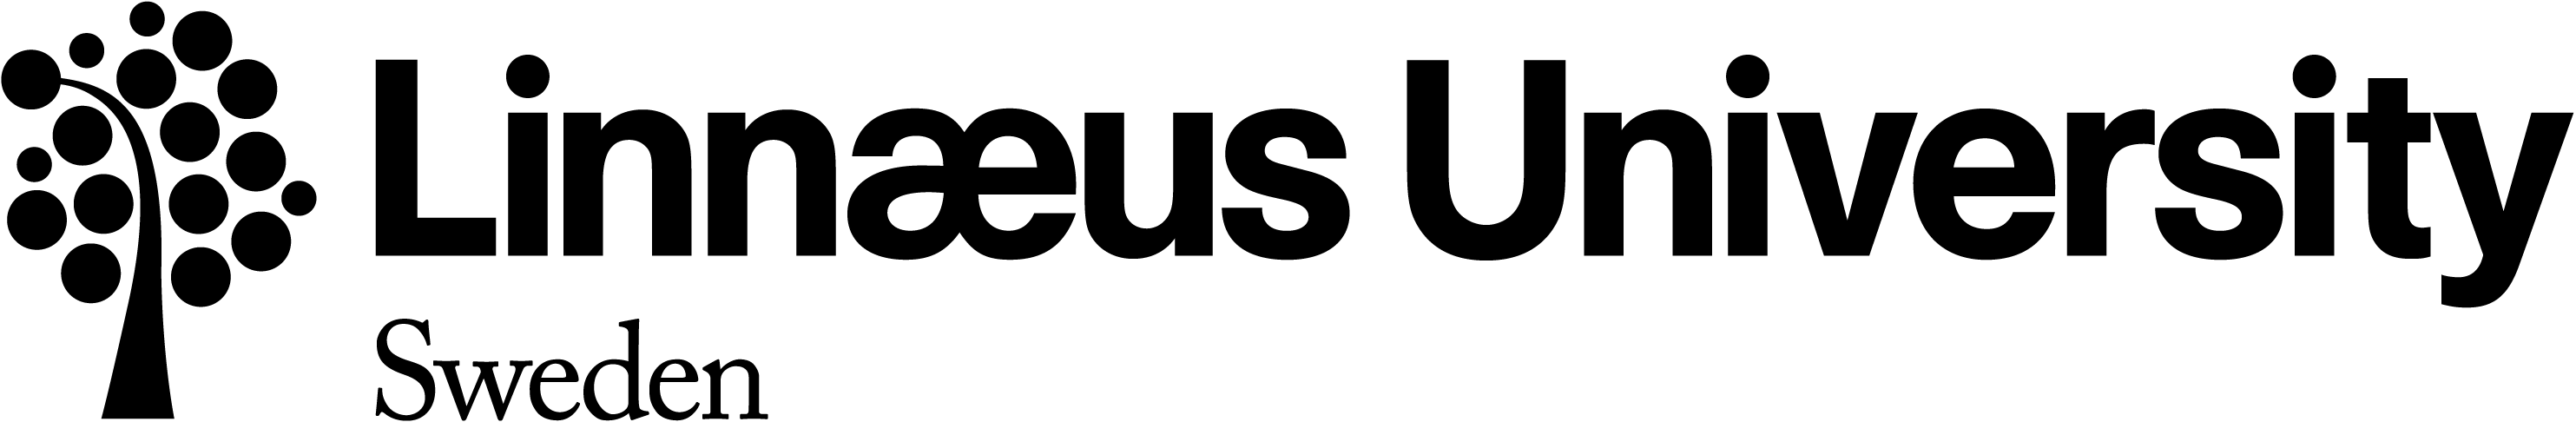
\includegraphics[width=.8\linewidth]{images/Lnu_Wordmark_Symbol_Sweden_Eng_rgb.png}
  \end{figure}
Department of Computer Science and Media Technology\\
Linnaeus University\\
Växjö, Sweden\\

\vspace{1.5cm}
\today


% More prosa about the university falala mcgill is so great.
\vspace{1.0cm}
\noindent
A thesis submitted to Linnaeus University in partial\\
fulfillment of the requirements of the degree of\\
Masters in Software Technology

% Add a copyright for your name, just in case.
\vspace{1.0cm}
{\small \copyright Prasannjeet Singh, \the\year{}}


\end{center}

\begin{tikzpicture}[remember picture,overlay]

    \node[anchor=south east, inner sep=0pt, xshift=-1cm, yshift=1cm] at (current page.south east) {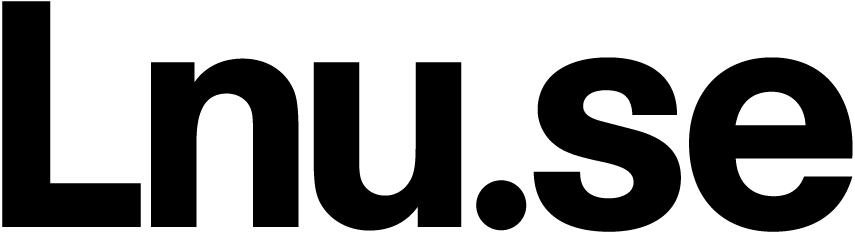
\includegraphics[width=2cm]{images/Lnu-se_rgb.png}};

    \node[anchor=south west, inner sep=0pt, xshift=-3cm, yshift=-1cm] at (current page.south west) {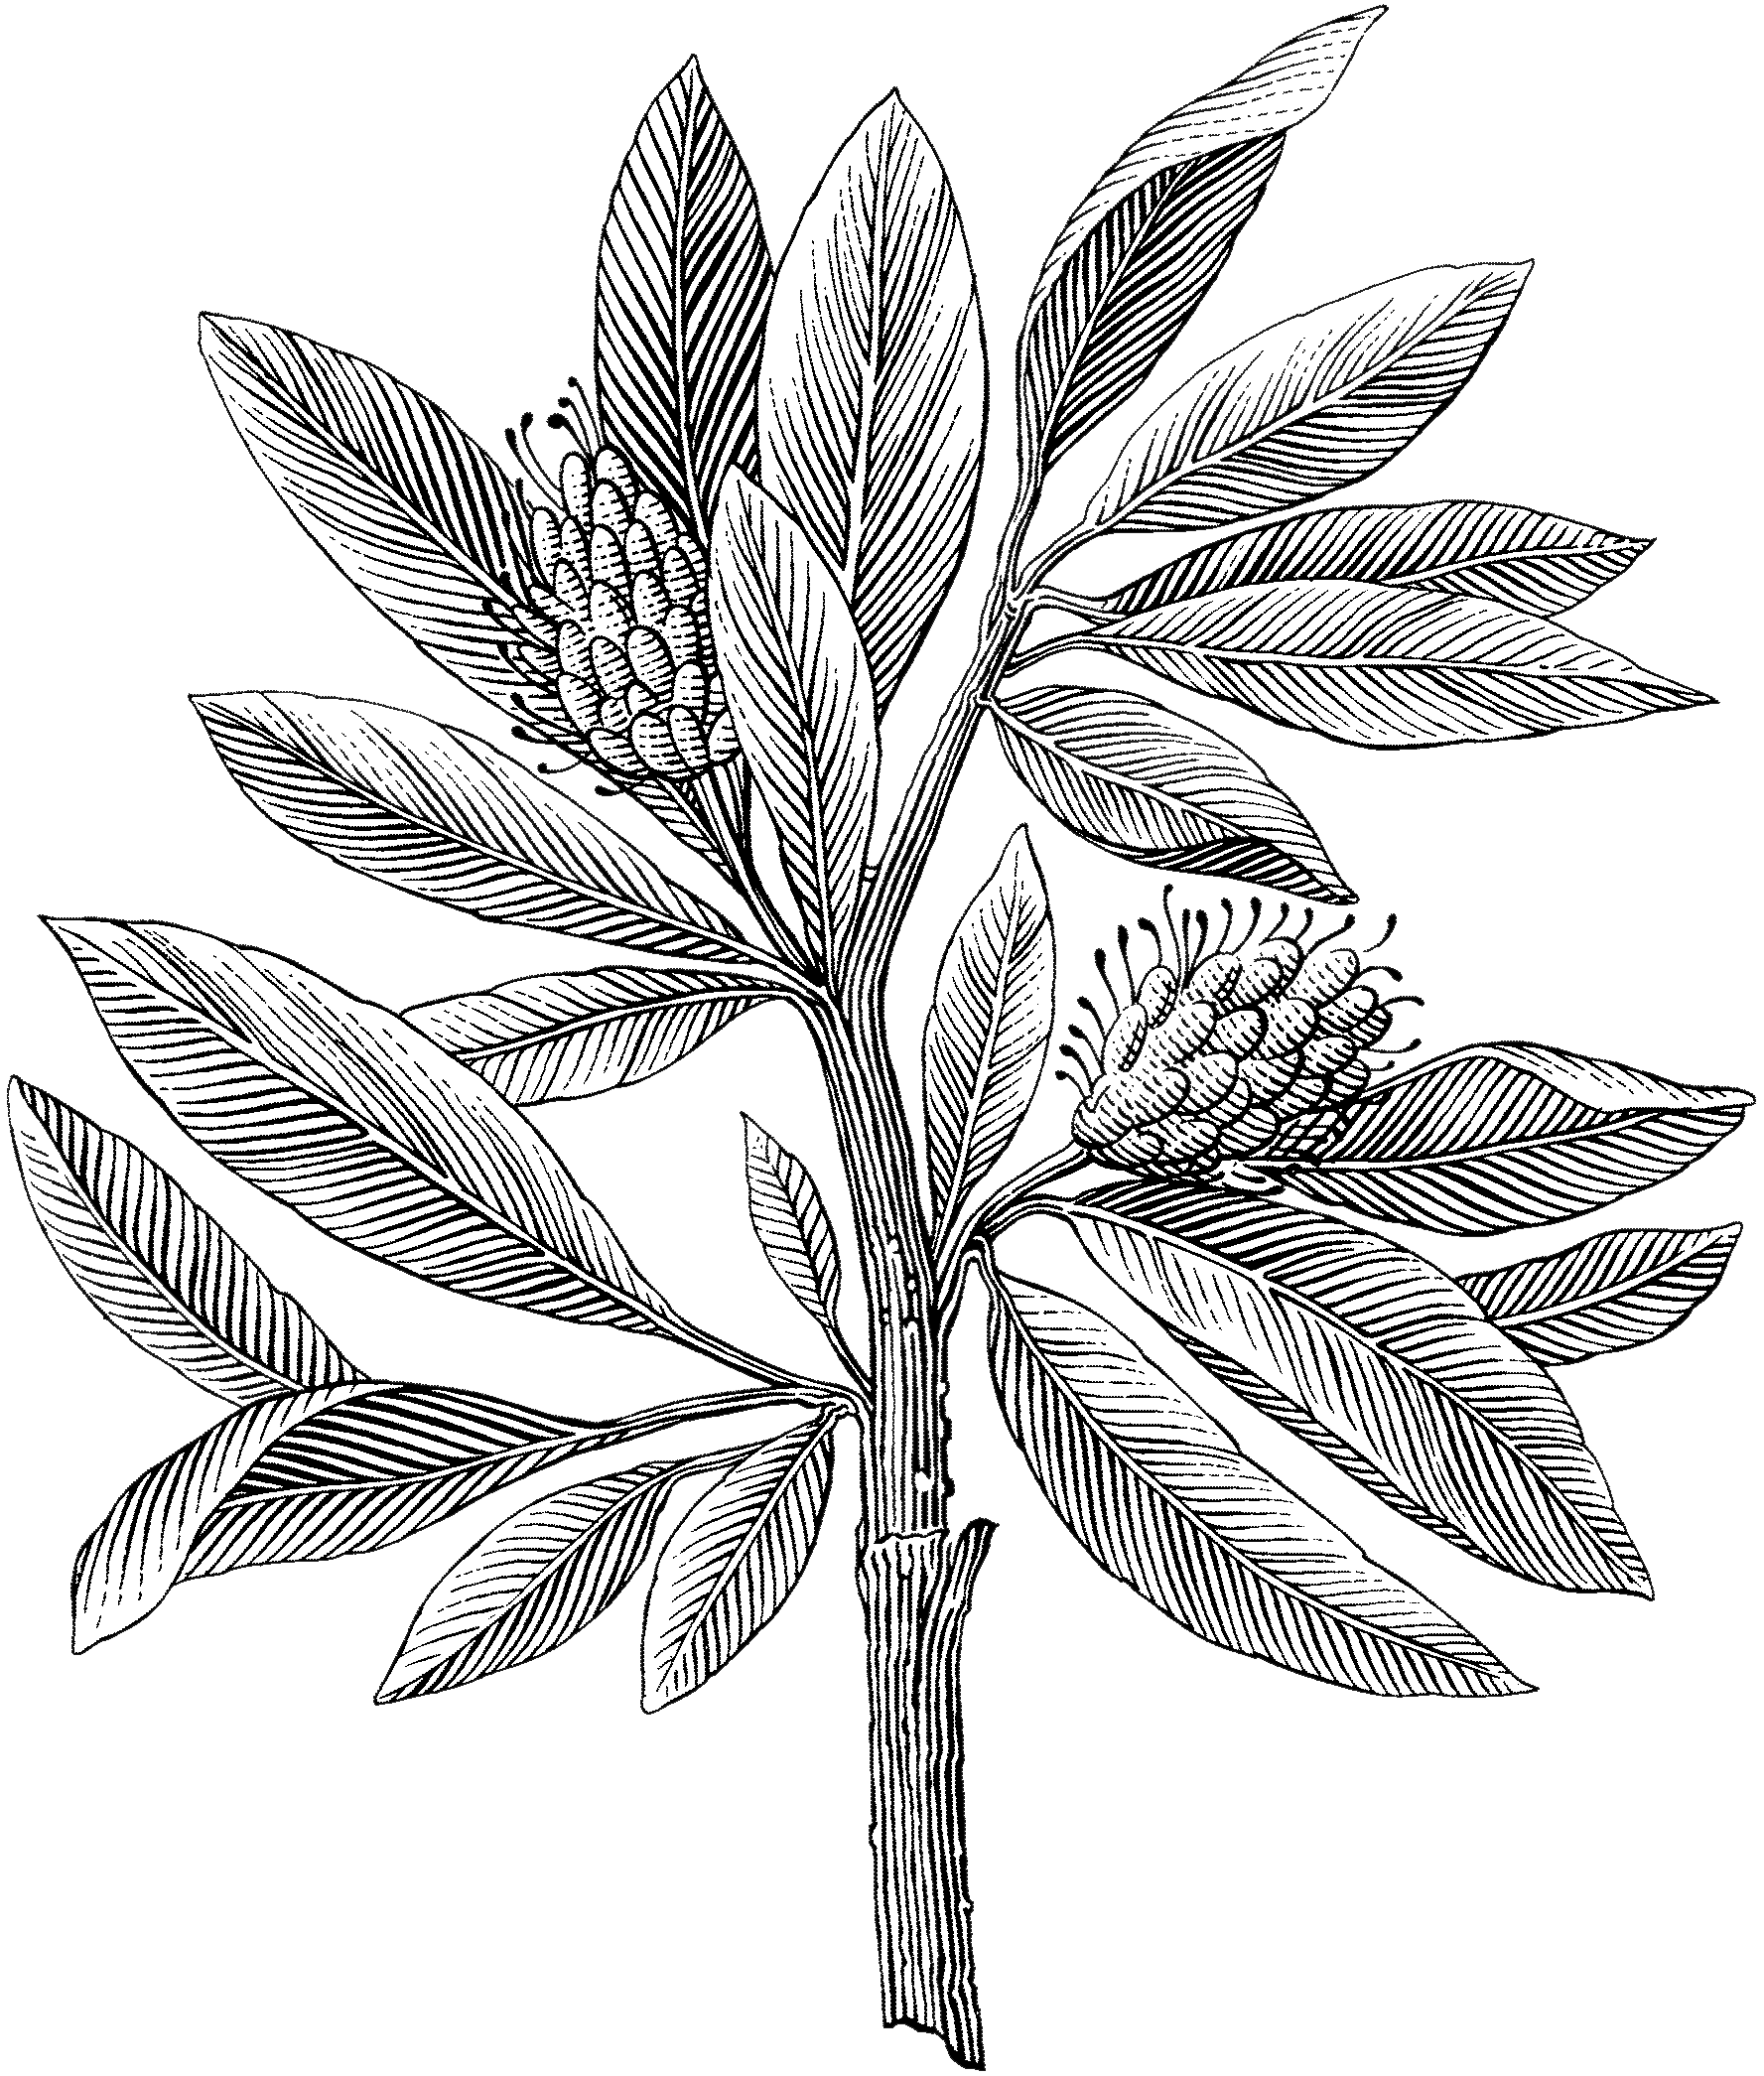
\includegraphics[width=10cm]{images/lnu_copperplate_inv.png}};

    \node[anchor=north west, inner sep=0pt, xshift=1cm, yshift=-1cm] at (current page.north west) {
\includegraphics[width=2.5cm]{images/logo_yellow.jpg}};
\end{tikzpicture}


\end{titlepage}






\cleardoublepage
\end{onehalfspacing}


% Pages in all "Chapters" before the actual thesis content are enumerated in roman (i, ii, iii, ...)
\pagenumbering{roman}
\pagestyle{plain}


% Abstracts in English and French
\chapter*{\rm\bfseries Abstract}
\label{ch:abstraten}

\href{https://www.mcgill.ca/gps/thesis/thesis-guidelines/preparation}{Official McGill Guidelines}: If the language of the thesis is neither English nor French (only allowed for specific language Units) then a third abstract in the language of the thesis is required.

Abstracts in English and French are mandatory and must be text only, i.e. no images, special characters (apart from the West European character set excluding the “Œ” and “œ”), chemical or mathematical formulae, or special formatting (e.g. lists, tables). Abstracts have a maximum limit of 4000 characters.
\clearpage
\chapter*{\rm\bfseries Abr\'eg\'e}
\label{ch:abstratfr}

\href{https://www.mcgill.ca/gps/thesis/thesis-guidelines/preparation}{Official McGill Guidelines}: La même chose en français.
\cleardoublepage


% List of Contributions
% Abstracts in English and French
\chapter*{\rm\bfseries Contribution}
\label{ch:contribution}

\href{https://www.mcgill.ca/gps/thesis/thesis-guidelines/preparation}{Official McGill Guidelines}: A doctoral thesis must clearly state the elements of the thesis that are considered original scholarship and distinct contributions to knowledge.

\begin{itemize}
    \item{Contributions of the student to each chapter must be explicitly stated.}
    \item{Contributions of any co-authors to each chapter must be explicitly stated.}
\end{itemize}


 
\clearpage


% Acknowledgements
\chapter*{\rm\bfseries Acknowledgements}
\label{ch:acknowledgement}

\href{https://www.mcgill.ca/gps/thesis/thesis-guidelines/preparation}{Official McGill Guidelines}: Among other acknowledgements, the student is required to declare the extent to which assistance (paid or unpaid) has been given by members of staff, fellow students, research assistants, technicians, or others in the collection of materials and data, the design and construction of apparatus, the performance of experiments, the analysis of data, and the preparation of the thesis (including editorial help).


\begin{itemize}
    \item{In addition, it is appropriate to recognize the supervision and advice given by the thesis supervisor(s) and advisors.}
\end{itemize}
\clearpage

% Next comes the GENERATED list of contents, figures and tables.
\tableofcontents
\listoffigures
\listoftables
\clearpage



% Here comes the actual thesis content, we switch back to arabic page numbers.
\pagenumbering{arabic}
% \pagestyle{fancyplain}


% Intro and literature are mandatory mcgill parts:
\chapter*{\rm\bfseries Introduction}
\label{ch:introduction}

\mcgillguidelines Clearly state the rationale and objectives of the research.


\chapter*{\rm\bfseries Literature}
\label{ch:literature}

\mcgillguidelines: The comprehensive review of the literature must sufficiently demonstrate the student’s knowledge of and expertise in their research areas and should be broad enough to apply to each research question in the thesis. The review of the literature can additionally include various types of content, such as:

\begin{itemize}
    \item{A review providing a reader who is relatively less familiar with the research topic (e.g., an internal/external member of an oral defence committee with adjacent but not direct expertise) an introduction to the general domain.}
    \item{An explanation of the overall rationale for how and why the subsequent studies were conducted. For example, the literature underlying the research questions must be sufficiently discussed.}
    \item{A review of fundamental theories underlying the subsequently presented work, or to explain why certain approaches were not taken in the study(ies) presented.}
\end{itemize}

The literature review must be in line with disciplinary expectations. The review can be incorporated in the Introduction chapter, addressed in a standalone chapter, or distributed across multiple chapters.

% Two sample parts with sample chapters, change this parts as much as your little heart desires:
\part{Why Does the Sun Shine?}
\label{part:part1}
\chapter{\rm\bfseries First Chapter Title Here}
\label{ch:chapter01}

Lorem ipsum dolor sit amet, consectetur adipiscing elit, sed do eiusmod tempor incididunt ut labore et dolore magna aliqua. Ut enim ad minim veniam, quis nostrud exercitation ullamco laboris nisi ut aliquip ex ea commodo consequat. Duis aute irure dolor in reprehenderit in voluptate velit esse cillum dolore eu fugiat nulla pariatur. Excepteur sint occaecat cupidatat non proident, sunt in culpa qui officia deserunt mollit anim id est laborum.


\chapter{\rm\bfseries Second Chapter Title Here}
\label{ch:chapter02}

Lorem ipsum dolor sit amet, consectetur adipiscing elit, sed do eiusmod tempor incididunt ut labore et dolore magna aliqua. Ut enim ad minim veniam, quis nostrud exercitation ullamco laboris nisi ut aliquip ex ea commodo consequat. Duis aute irure dolor in reprehenderit in voluptate velit esse cillum dolore eu fugiat nulla pariatur. Excepteur sint occaecat cupidatat non proident, sunt in culpa qui officia deserunt mollit anim id est laborum.



\part{Why Does the Sun Really Shine?}
\label{part:part2}
\chapter{\rm\bfseries Third Chapter Title Here}
\label{ch:chapter03}

Lorem ipsum dolor sit amet, consectetur adipiscing elit, sed do eiusmod tempor incididunt ut labore et dolore magna aliqua. Ut enim ad minim veniam, quis nostrud exercitation ullamco laboris nisi ut aliquip ex ea commodo consequat. Duis aute irure dolor in reprehenderit in voluptate velit esse cillum dolore eu fugiat nulla pariatur. Excepteur sint occaecat cupidatat non proident, sunt in culpa qui officia deserunt mollit anim id est laborum.


% more chapters here, you get the idea...


% Finally, as you reach the end of your thesis: (Discussion is a mandatory part, see mcgill guidelines:
% https://www.mcgill.ca/gps/thesis/thesis-guidelines/preparation
\part{Discussion and Conclusions}
\label{part:disclusions}
\chapter{\rm\bfseries Discussion}
\label{ch:discussion}

\mcgillguidelines The discussion of findings must be in line with disciplinary expectations. A comprehensive discussion is expected to be a minimum of 10 pages, double-spaced for doctoral students and a minimum of 5 pages, double-spaced for Master’s students (including figures, images, and tables). It pertains to the entirety of a thesis. The discussion of findings should provide an final, overarching summary of study themes, limitations, and future directions.


In the case of a manuscript-based thesis, the comprehensive discussion should encompass all of the chapters of the thesis and should not be a repetition of the individual chapters. This section can be used to address issues not sufficiently covered in the preceding chapters or papers (e.g., critiques raised by reviewers that could not be incorporated into published works, or reintroducing discussion arguments removed from published papers upon reviewer request). This section can also be used to elaborate on the practical/applied aspects of published findings in a manner that is more accessible to less expert readers.
\chapter{\rm\bfseries Conclusions and Future Work}
\label{ch:conclusions}

\mcgillguidelines Clearly state how the objectives of the research were met and discuss implications of findings.




% If you want to mention future work, pack it here.


% List of YOUR publications
\chapter*{\rm\bfseries Publications}
\label{ch:publications}

This part is optional, but it gives a nice touch to list all the publications (official venues down to poster sessions) throughout your PhD.

Keep this in the same style as publications in your academic CV: 
Conference / Year - Title - Authors. And here comes a sample ref for the bibliography: \cite{schiedermeier_fiddlr_2021} and \cite{schiedermeier_fiddlr_2021} and finally \cite{schiedermeier_fiddlr_2021}.



% Optional: List of Acronyms / Glossary
\chapter*{\rm\bfseries Acronyms}
\label{ch:acronyms}

This part is likewise optional. But it does not hurt to provide a list of all acronyms, e.g.:

\begin{itemize}
    \item{\textbf{REST}: \textbf{Re}presentational \textbf{S}tate \textbf{T}ransfer}
\end{itemize}


% Finally your references
% PLEASE use a management system, e.g. Zotero (this works really nice with overleaf, there's seamless referencing of all your organized papers from zotero).
% To add zotero, use "New file -> From Zotero"
\bibliographystyle{alpha}
\bibliography{references}

\end{document}